\documentclass{beamer}

\usepackage{graphicx}

\usecolortheme[named=blue]{structure}

\mode<presentation>
{
  \usetheme{Warsaw}
  \setbeamercovered{transparent}
  \setbeamertemplate{items}[ball]
  \setbeamertemplate{theorems}[numbered]
  \setbeamertemplate{footline}[frame number]
  
% custom colors
  \setbeamercolor{structure}{fg=red!90!black}
  
  \setbeamerfont{section number projected}{%
  	family=\rmfamily,series=\bfseries,size=\normalsize
  }
  \setbeamercolor{section number projected}{bg=red,fg=white}
  
}

% \usecolortheme{spruce}

\usepackage{beamerthemesplit}
\usepackage{graphics}
\usepackage{graphicx}
\usepackage{hyperref}
\usepackage{color}
\usepackage{listings}
\usepackage[utf8]{inputenc}

\newcommand{\code}[1]{\texttt{\small{#1}}}
\hypersetup{%
  colorlinks=true,
  urlcolor=red,
  linkcolor=red,
  pdfborderstyle={/S/U/W 1}
}

\definecolor{javared}{rgb}{0.6,0,0} % for strings
\definecolor{javagreen}{rgb}{0.25,0.5,0.35} % comments
\definecolor{javapurple}{rgb}{0.5,0,0.35} % keywords
\definecolor{javadocblue}{rgb}{0.25,0.35,0.75} % javadoc

\lstdefinelanguage{scala}{
  morekeywords={abstract,case,catch,class,def,%
    do,else,extends,false,final,finally,%
    for,if,implicit,import,match,mixin,%
    new,null,object,override,package,%
    private,protected,requires,return,sealed,%
    super,this,throw,trait,true,try,%
    type,val,var,while,with,yield},
  otherkeywords={=>,<-,<\%,<:,>:,\#,@,>,<},
  sensitive=true,
  morecomment=[l]{//},
  morecomment=[n]{/*}{*/},
  morestring=[b]",
  morestring=[b]',
  morestring=[b]"""
}
\lstset{
%   frame=tb,
  language=Scala,
  aboveskip=3mm,
  belowskip=3mm,
  columns=flexible,
  basicstyle=\ttfamily\small,
  keywordstyle=\color{javapurple}\bfseries,
  stringstyle=\color{javared},
  commentstyle=\color{javagreen},
  morecomment=[s][\color{javadocblue}]{/**}{*/},
  numbers=none,
  numberstyle=\tiny\color{black},
  stepnumber=2,
  numbersep=10pt,
  showspaces=false,
  showstringspaces=false,
  tabsize=4
}

\newcommand{\screenshot}[1]{\centerline{%
    \includegraphics[height=7.8cm,transparent]{#1}}}  % 7.8in

\title
  [Wollok: en el aula y más allá]
  {Wollok: en el aula y más allá}
\author[Passerini, Fernandes, Tesone]{%
  Javier Fernandes\inst{1,2} \and
  Nicolás Passerini\inst{1,2,4} \\
  Pablo Tesone\inst{3,1,2,4} \and
  Débora Fortini\inst{1,4} \\
  Nahuel Palumbo\inst{4} \and
  Juan Contardo\inst{4} \and
  Carlos Raffellini\inst{4}
}  

\institute{
  \inst{1}Universidad Nacional de Quilmes \\
  \inst{2}Universidad Nacional de San Martin \\
  \inst{3}Universidad Nacional del Oeste \\
  \inst{4}Universidad Tecnológica Nacional - F.R. Buenos Aires.
}

\date[WISIT 2015]{\small Workshop de Ingeniería en Sistemas y Tecnologías de la Información \\ 19/09/2015}
\subject{Computational Sciences}

%\logo{\includegraphics[height=1.0cm]{fsu_logo.pdf}}

\begin{document}
  \frame
  {
    \titlepage
  }

  \frame
  {
    \frametitle{Agenda}
    \tableofcontents
  }

\section{Introduccion}
\frame{
	\frametitle{¿Qué es Wollok?}
	// TODO introducir un toque wollok
	// seria bueno algún screenshot también	
}

\section{Desarrollo de Wollok}
\frame{
	\frametitle{Desarrollo de Wollok}	
	\begin{itemize}
		\item OpenSource: LGPLv3 
		\item Stack: Eclipse XText + Xtend Lang
		\item SCM:
			\begin{itemize}
			  	\item \textbf{Código}: GitHub
			  	(\href{https://github.com/uqbar-project/wollok}{uqbar-project/wollok})
			 	\item \textbf{Build}: Maven + Tycho
			 	\item \textbf{Continuous Integration}: Travis
			 	\item \textbf{Continuous Deployment}
			 	\item \textbf{Coverage}: coveralls + jacoco
			 \end{itemize}
		\item Testing \& TDD
	\end{itemize}
}

\frame{
	\frametitle{Desarrollo de Wollok}
	\framesubtitle{Continuous Integration \& Deployment}	
	\begin{itemize}
	  	\item \textbf{GitFlow}
	  		\begin{itemize}
	  		  \item Feature Branches
	  		  \item Pull-Requests
	  		  \item $dev \rightarrow master \leftarrow  hotfixes$ 
			\end{itemize}	 
		\item \textbf{Integration}:
			\begin{itemize}
			  \item Travis
			  \item compile, test, coverage, deploy
			\end{itemize}
		\item Deployment:
				\begin{itemize}
				  \item \textbf{Productos} (IDE): multiples pataformas
				  \item \textbf{Update Sites}
				  \item \textbf{WDK}
				  \item 2 Ambientes: Stable \& Dev
				\end{itemize}
	\end{itemize}
}

\frame{
	\frametitle{Desarrollo de Wollok}
	\framesubtitle{Testing \& TDD}	
	\begin{itemize}
	  	\item 87\% Cobertura 	
	  	\item \textbf{Runtime}      % SCREEN: ACA MOSTRAMOS UN SCREENSHOT DE UN TEST
	  		\begin{itemize}
	  		  \item Testean ejecución
	  		  \item Interprete
	  		  \item \textbf{JUnit + iDSL}
			\end{itemize}	 
		\item \textbf{Estáticos}
			\begin{itemize}
			  \item \textbf{Chequeos}: XPect  % SCREEN: ACA MOSTRAMOS UN TEXT XPECT
			  \item \textbf{Type System}: JUnit + iDSL
			  \item \textbf{Autocomplete}: XPect
			  \item \textbf{Formateo}: JUnit + iDSL
			\end{itemize}
		\item \textbf{Pendientes}
			\begin{itemize}
			  \item Quick-Fixes
			  \item Refactors
			\end{itemize}
	\end{itemize}
}

\frame{
	\frametitle{Testing \& TDD}
	\framesubtitle{Runtime}
	Testeo del intérprete
	\begin{center}
		\begin{figure}
			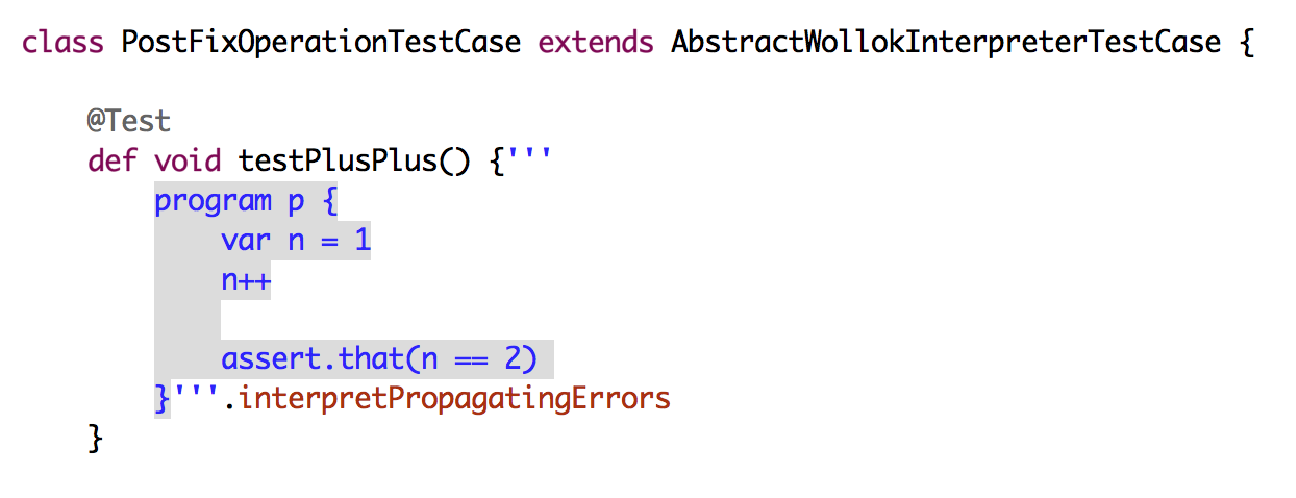
\includegraphics[height=0.8\textheight,natwidth=1212,natheight=446]{images/wollok-tests-runtime.eps}
		\end{figure}
	\end{center}
}

\frame{
	\frametitle{Testing \& TDD}
	\framesubtitle{Chequeos Estáticos}
	Testeo de Chequeos Estáticos
	\begin{center}
		\begin{figure}
			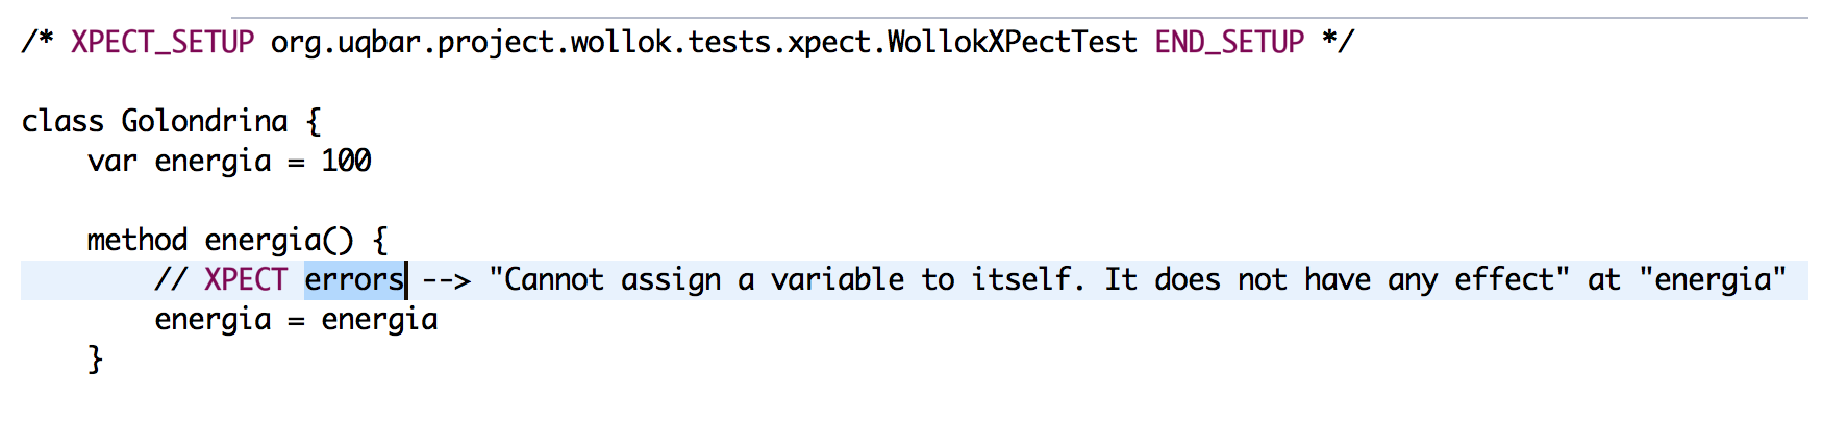
\includegraphics[height=0.8\textheight,natwidth=1720,natheight=372]{images/wollok-tests-checkeos.eps}
		\end{figure}
	\end{center}
}

\frame{
	\frametitle{Testing \& TDD}
	\framesubtitle{Autocomplete}
	Testeo del Autocomplete
	\begin{center}
		\begin{figure}
			\includegraphics[height=0.8\textheight,natwidth=2106,natheight=398]{images/wollok-tests-autocomplete.eps}
		\end{figure}
	\end{center}
}

\frame{
	\frametitle{Testing \& TDD}
	\framesubtitle{Formatter}
	Testeo del Formatter
	\begin{center}
		\begin{figure}
			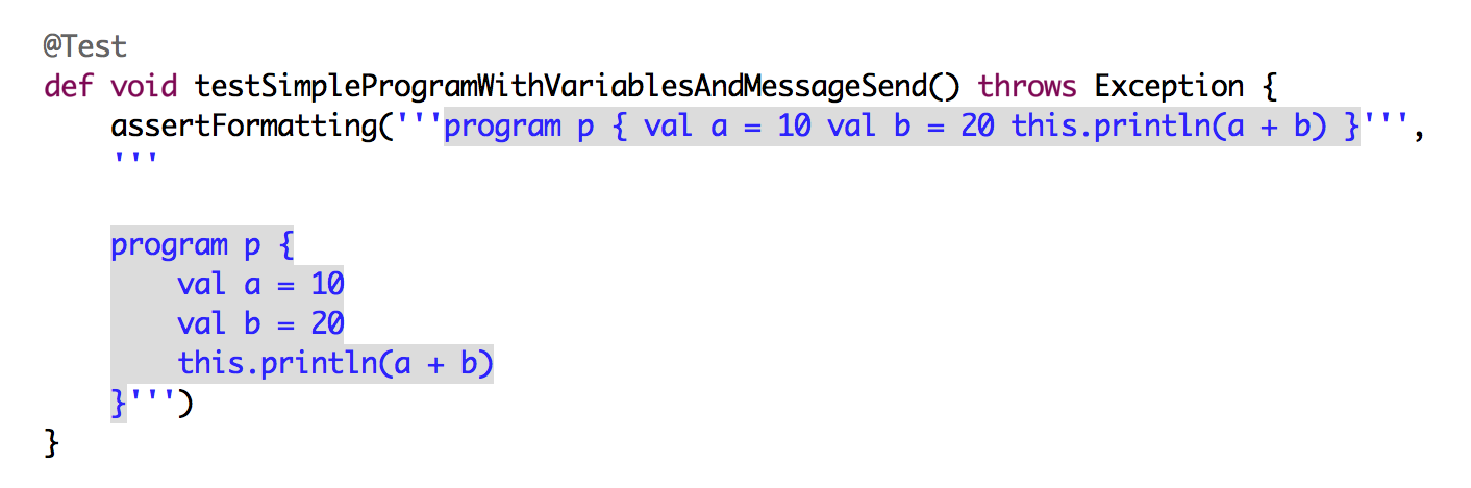
\includegraphics[height=0.8\textheight,natwidth=1380,natheight=436]{images/wollok-tests-formatter.eps}
		\end{figure}
	\end{center}
}

\frame{
	\frametitle{Testing \& TDD}
	\framesubtitle{Type System}
	Testeo del Type System
	\begin{center}
		\begin{figure}
			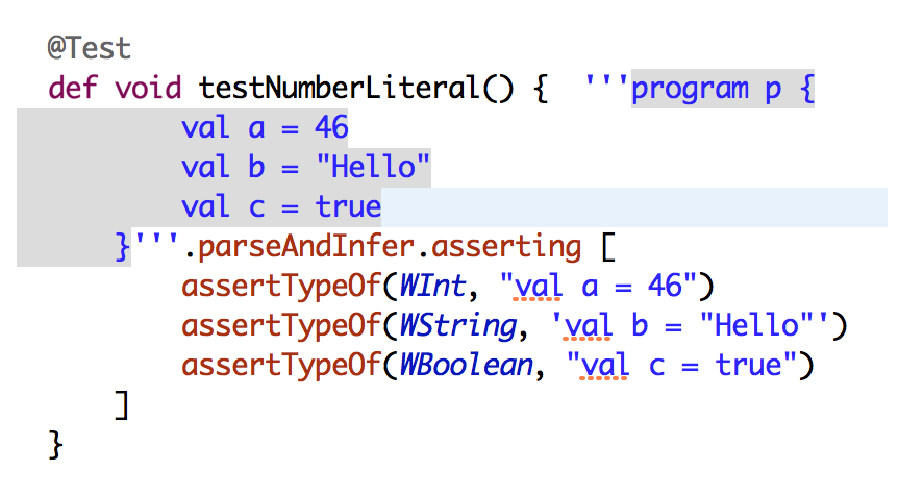
\includegraphics[height=0.8\textheight,natwidth=836,natheight=444]{images/wollok-tests-typesystem.eps}
		\end{figure}
	\end{center}
}

%
% FEATURE AVANZADOS
%

\section{Features Avanzados}
\frame{
	\frametitle{Features Avanzados}	
	\begin{itemize}
    \item Debugger
    \item Tests
    \item Sublime Plugins 
    \item I18N
	\end{itemize}
}

\frame{
	\frametitle{Debugger}
	\begin{itemize}
	    \item UI integrada a Eclipse Debug
	    \item Breakpoints: agregar, remover, deshabilitar, etc
	    \item Step, into, out 
	    \item Inspeccionar variables
	\end{itemize}
}


\frame{
	\frametitle{Sublime Support}	
	\begin{itemize}
	    \item WDK
	    	\begin{itemize}
	    		\item No IDE
	    		\item $\sim70$MB (vs $\sim140$)
	    		\item Headless: wchecker, winterpreter, wtest
	    	\end{itemize}
	    \item Syntax highlight
	    \item Templates 
	    \item Linter
	\end{itemize}
}


\frame{
	\frametitle{Sublime Support}
	\framesubtitle{Syntax Highlight}	
	\begin{center}
		\begin{figure}
			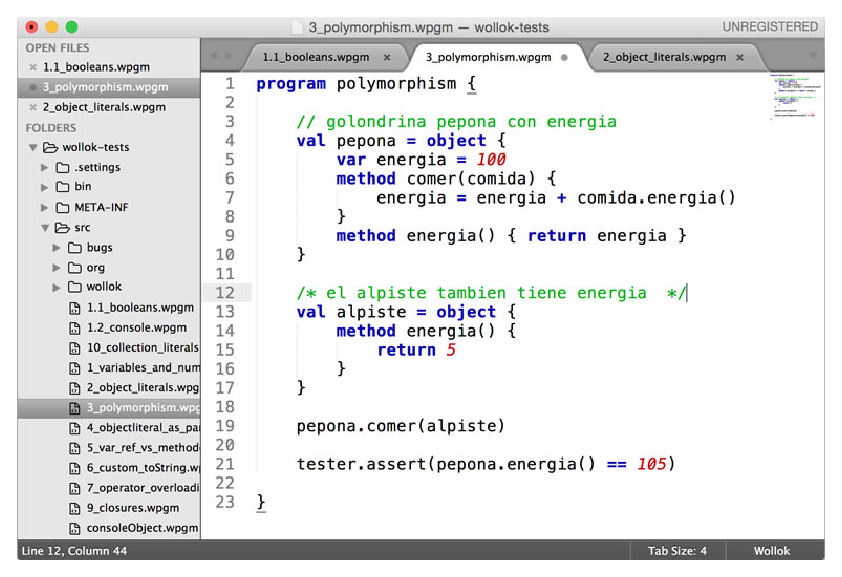
\includegraphics[height=0.8\textheight,natwidth=800,natheight=561]{images/wollok-wisit-sublime-syntax.eps}
		\end{figure}
	\end{center}
}

\frame{
	\frametitle{Sublime Support}
	\framesubtitle{Linter}
	\begin{center}
		\begin{figure}
			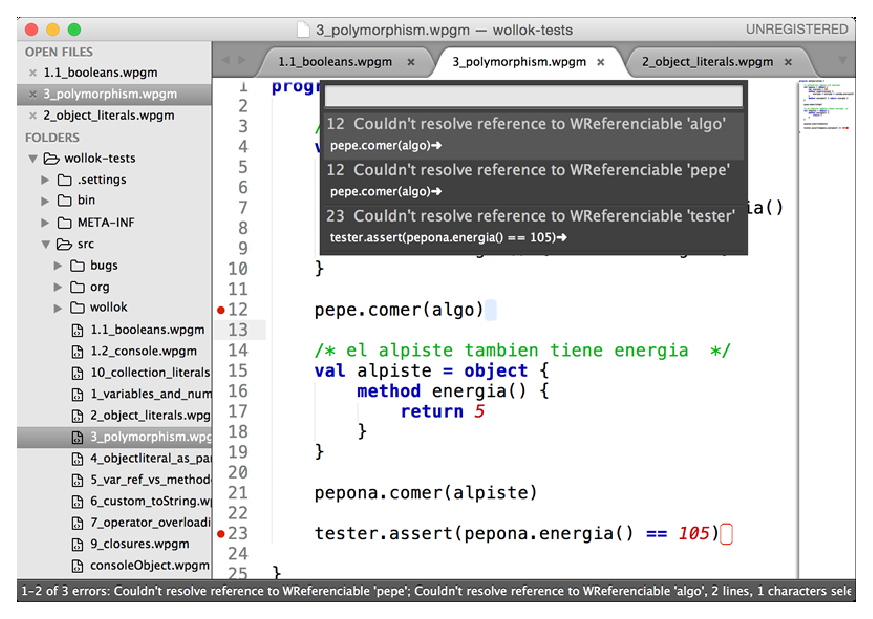
\includegraphics[height=0.8\textheight,natwidth=800,natheight=558]{images/wollok-wisit-sublime-linter.eps}
		\end{figure}
	\end{center}
}


%
% WOLLOK GAME
%

\section{Wollok Game}
\frame{
	\frametitle{Wollok Game}
	\begin{itemize}
		\item s
		\item a
		\item b
		\item o
	\end{itemize}
}

\section{Experiencia en el Aula}
\frame{
	\frametitle{Experiencia en el Aula}	
	\begin{itemize}
		\item s
		\item a
		\item s
	\end{itemize}
}


\frame{
  \frametitle{Muchas gracias}.
}
\end{document}

